%%%%%%%%%%%%%%%%%%%%%%%%%%%%%%%%%%%%%
%                                   %
% Compile with XeLaTeX and biber    %
%                                   %
% Questions or comments:            %
%                                   %
% joshua dot mcneill at uga dot edu %
%                                   %
%%%%%%%%%%%%%%%%%%%%%%%%%%%%%%%%%%%%%

\documentclass{beamer}
  % Read in standard preamble (cosmetic stuff)
  %%%%%%%%%%%%%%%%%%%%%%%%%%%%%%%%%%%%%%%%%%%%%%%%%%%%%%%%%%%%%%%%
% This is a standard preamble used in for all slide documents. %
% It basically contains cosmetic settings.                     %
%                                                              %
% Joshua McNeill                                               %
% joshua dot mcneill at uga dot edu                            %
%%%%%%%%%%%%%%%%%%%%%%%%%%%%%%%%%%%%%%%%%%%%%%%%%%%%%%%%%%%%%%%%

% Beamer settings
% \usetheme{Berkeley}
\usetheme{CambridgeUS}
% \usecolortheme{dove}
% \usecolortheme{rose}
\usecolortheme{seagull}
\usefonttheme{professionalfonts}
\usefonttheme{serif}
\setbeamertemplate{bibliography item}{}

% Packages and settings
\usepackage{fontspec}
  \setmainfont{Charis SIL}
\usepackage{hyperref}
  \hypersetup{colorlinks=true,
              allcolors=blue}
\usepackage{graphicx}
  \graphicspath{{../../figures/}}
\usepackage[normalem]{ulem}
\usepackage{enumerate}

% Document information
\author{M. McNeill}
\title[FREN2001]{Français 2001}
\institute{\url{joshua.mcneill@uga.edu}}
\date{}

%% Custom commands
% Lexical items
\newcommand{\lexi}[1]{\textit{#1}}
% Gloss
\newcommand{\gloss}[1]{`#1'}
\newcommand{\tinygloss}[1]{{\tiny`#1'}}
% Orthographic representations
\newcommand{\orth}[1]{$\langle$#1$\rangle$}
% Utterances (pragmatics)
\newcommand{\uttr}[1]{`#1'}
% Sentences (pragmatics)
\newcommand{\sent}[1]{\textit{#1}}
% Base dir for definitions
\newcommand{\defs}{../definitions}


  % Packages and settings

  % Document information
  \subtitle[Pays et prépositions]{Les pays et les prépositions}

\begin{document}
  % Read in the standard intro slides (title page and table of contents)
  \begin{frame}
    \titlepage
    \tiny{Office: % Basically a variable for office hours location
Gilbert 121\\
          Office hours: % Basically a variable for office hours
 lundi, mercredi, vendredi 10:10--11:10
}
  \end{frame}

  \begin{frame}{Dans quel pays?}
    \footnotesize
    \begin{columns}
      \column{0.5\textwidth}
        \begin{enumerate}
          \item On mangera du sushi, et on pourra prendre des trains super rapides.
          \item<2->[$\to$] On ira au Japon.
          \item<3-> Nous boirons un cappuccino, et nous regardons les gondoles qui passent.
          \item<4->[$\to$] Nous irons en Italie.
          \item<5-> Là-bas, je trouverai l'administration centrale de l'Union européenne.
          \item<6->[$\to$] J'irai en Belgique.
          \item<7-> C'est le seul pays d'Europe où vous pourrez parler espagnol.
          \item<8->[$\to$] Vous irez en Espagne.
        \end{enumerate}
      \column{0.5\textwidth}
        \begin{minipage}[c][0.8\textheight]{\linewidth}
          \begin{center}
            \only<2>{
              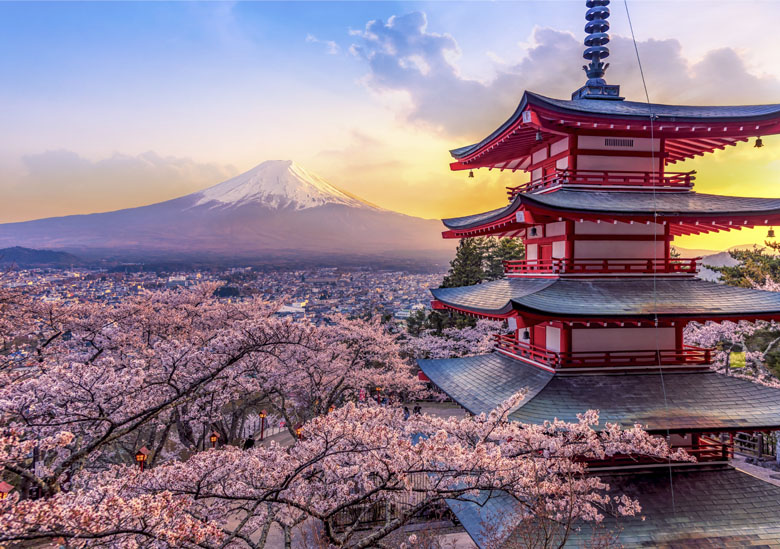
\includegraphics[scale=0.9]{japon.jpg}
            }
            \only<4>{
              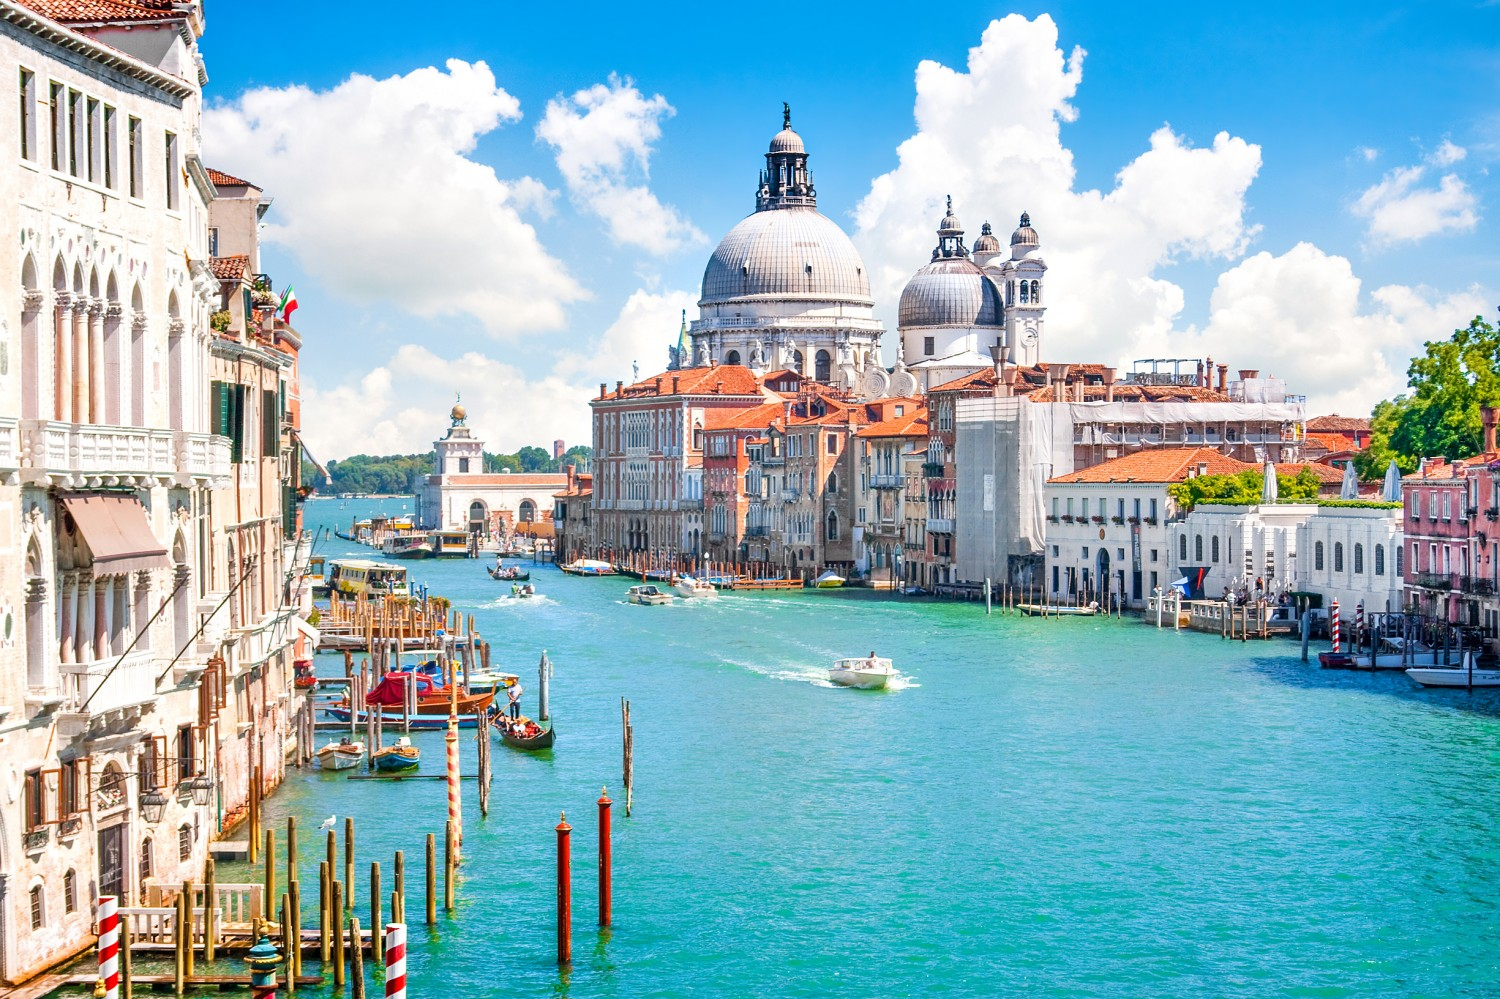
\includegraphics[scale=0.115]{italie.jpg} \\
              Veni\alert{s}e
            }
            \only<6>{
              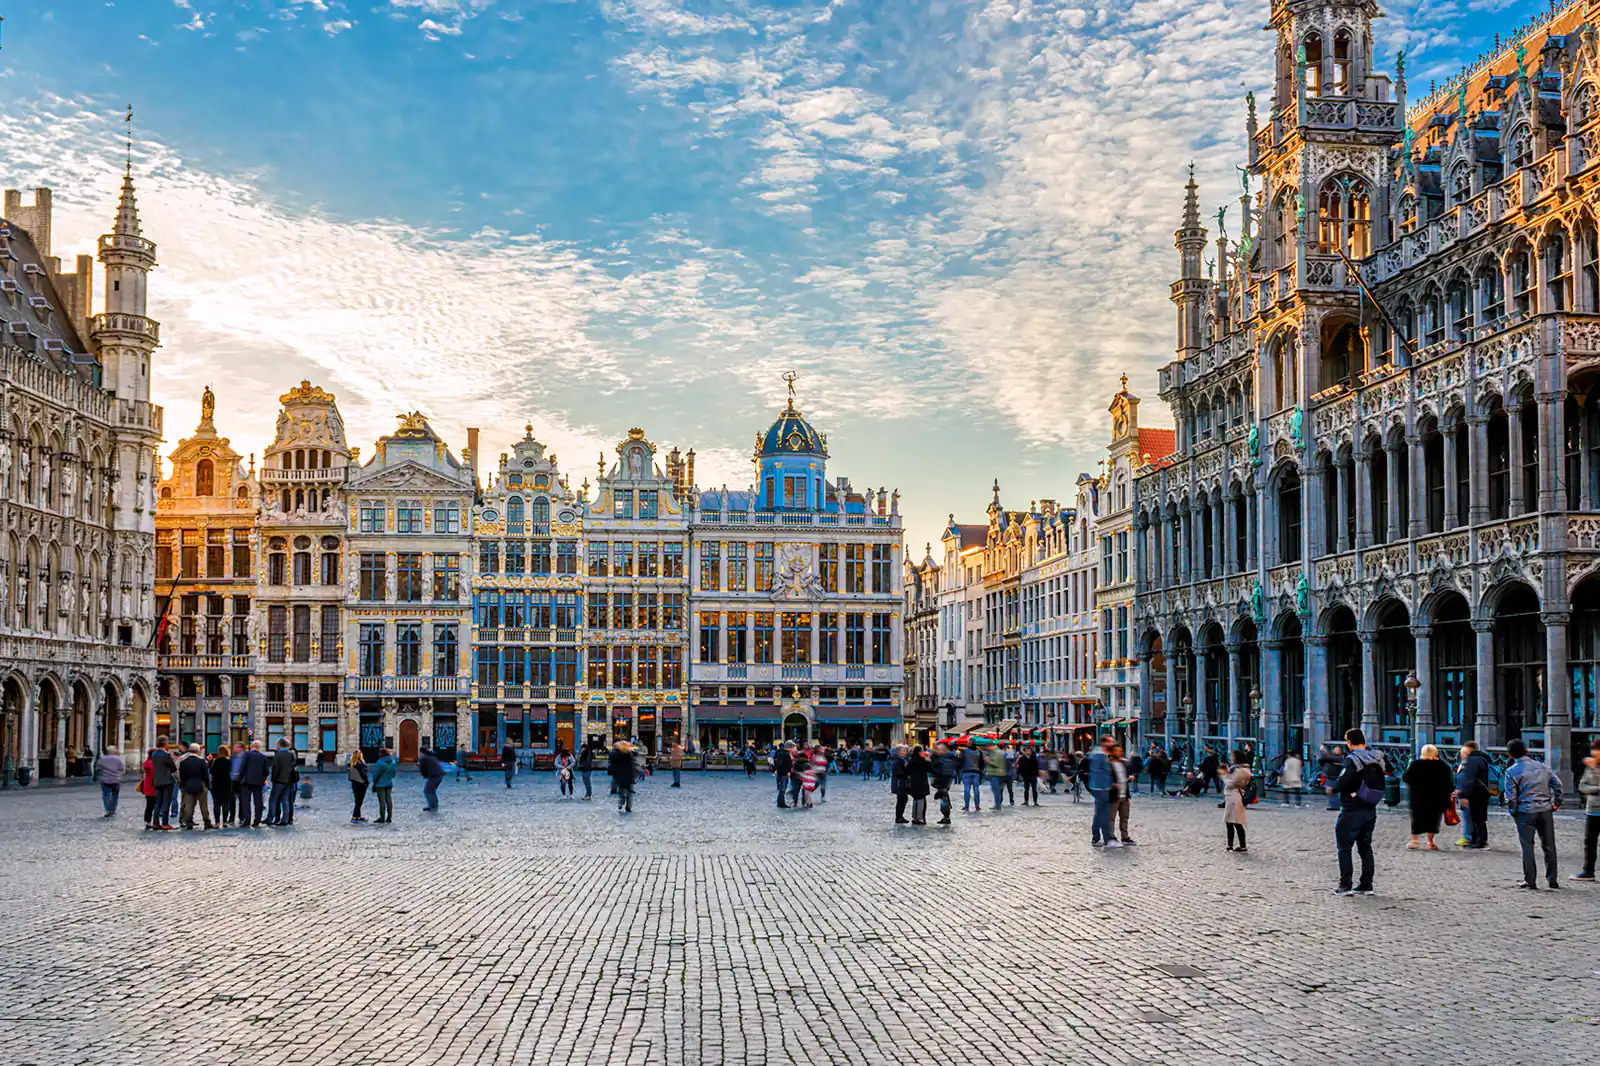
\includegraphics[scale=0.105]{belgique.jpg} \\
              La Grand-Place de Bruxelles
            }
            \only<8>{
              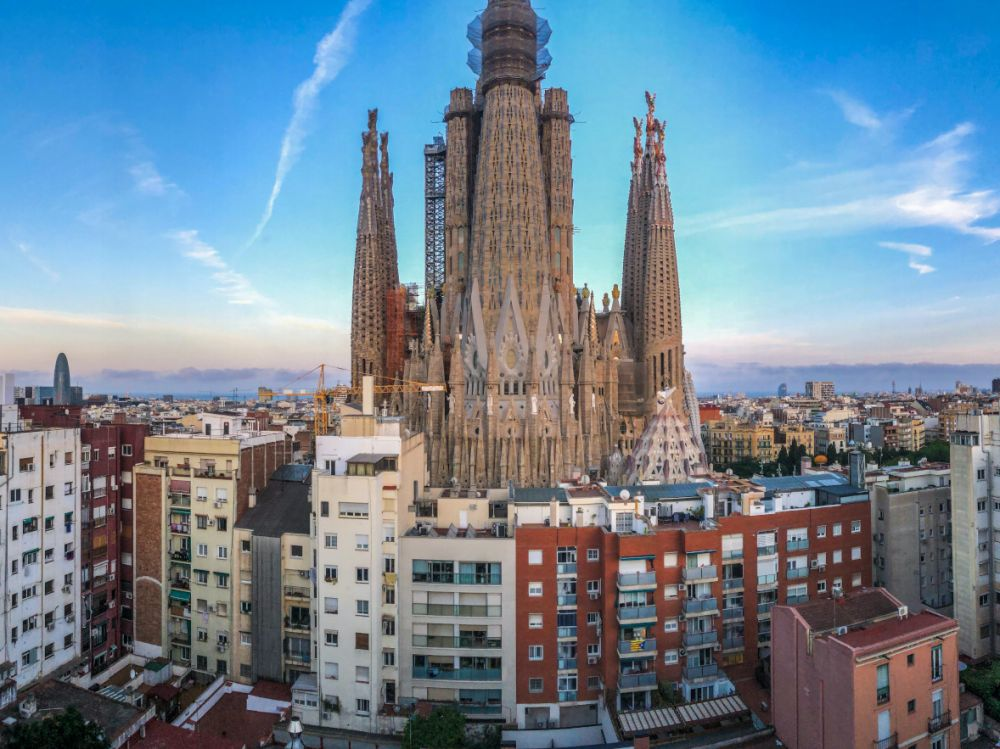
\includegraphics[scale=0.22]{espagne.jpg} \\
              La Sagrada Família (1882-présent) -- Antoni Gaudí
            }
          \end{center}
        \end{minipage}
    \end{columns}
  \end{frame}

  \begin{frame}{}
    \begin{center}
      \Large Quiz
    \end{center}
  \end{frame}

  \begin{frame}{Liaisons obligatoires}
    Est-ce que j'ai prononcé une liaison ou non?
    \begin{enumerate}
      \item \textcolor<13->{red}{les hôtels} \underline{\uncover<2->{oui}}
      \item<3-> \textcolor<13->{red}{leurs enfants} \underline{\uncover<4->{oui}}
      \item<5-> \textcolor<13->{red}{nous habitons} \underline{\uncover<6->{oui}}
      \item<7-> \textcolor<13->{red}{aux Antilles} \underline{\uncover<8->{oui}}
      \item<9-> pas encore \underline{\uncover<10->{non}}
      \item<11-> ils ont payé \underline{\uncover<12->{non}}
    \end{enumerate}
    \uncover<13->{
      \textcolor{red}{Ce sont des liaisons vraiment obligatoires.}
    }
  \end{frame}

  \begin{frame}{Liaisons à part de /z/}
    Est-ce que j'ai prononcé une liaison ou non?
    \begin{enumerate}
      \item un hôtel \underline{\uncover<2->{oui}}
      \item<3-> mon église \underline{\uncover<4->{oui}}
      \item<5-> il en a \underline{\uncover<6->{oui}}
      \item<7-> un petit animal \underline{\uncover<8->{oui}}
      \item<9-> ils sont ici \underline{\uncover<10->{non}}
    \end{enumerate}
  \end{frame}

  \begin{frame}{Un pays lointain}
    Avec un/e partenaire, imagine que tu pars visiter un autre pays.
    Quel pays est-ce que tu choisiras?
    Qu'est-ce que tu y feras?
    Discutes-en avec ton/ta partenaire.
    \begin{description}
      \item[] \textbf{Modèle:}
      \item[E1:] Je visiterai la Suisse, \alert{parce que} j'ai des cousins là-bas. Je ferai du ski dans les Alpes.
      \item[E2:] Est-ce tu as déjà fait du ski dans les Alpes avant?
      \item[E1:] Non, jamais, mais je fais du ski tous les ans. Et toi? Où est-ce que tu iras?
      \item[E2:] Moi, j'irai en Égypte. J'irai voir les pyramides.
      \item[E1:] Est-ce que tu étudies l'histoire?
      \item[E2:] Oui! Je l'étudie, particulièrement l'histoire ancienne.
    \end{description}
  \end{frame}

  \begin{frame}{}
    \begin{center}
      \Large Questions?
    \end{center}
  \end{frame}
\end{document}
